\chapter{Deep Gated Multimodal Units} \label{chap:deepgmu}

In this chapter we propose a novel multimodal fusion approach to integrate information from multiple genomic sources. While most methods have solely relied on data level fusion (early fusion) or decision level fusion (late fusion), our approach utilizes a series of cascading gated multimodal units to deeply connect the integration of data fusion and decision fusion.
%by a series of cascading layers

\section{Architecture}

The deep gated multimodal unit (dGMU) first contains multiplicative gates designed to construct an intermediate representation of data from multiple modalities. The input modalities along with the intermediate representation are then fed to a decision network that fuses the predictions using an additional gate. These two processes can be subdivided into the function of a representation network and a decision network. This structure is illustrated in Fig. \ref{fig:dgmu}. 

\begin{figure}[h!]
    \centering
    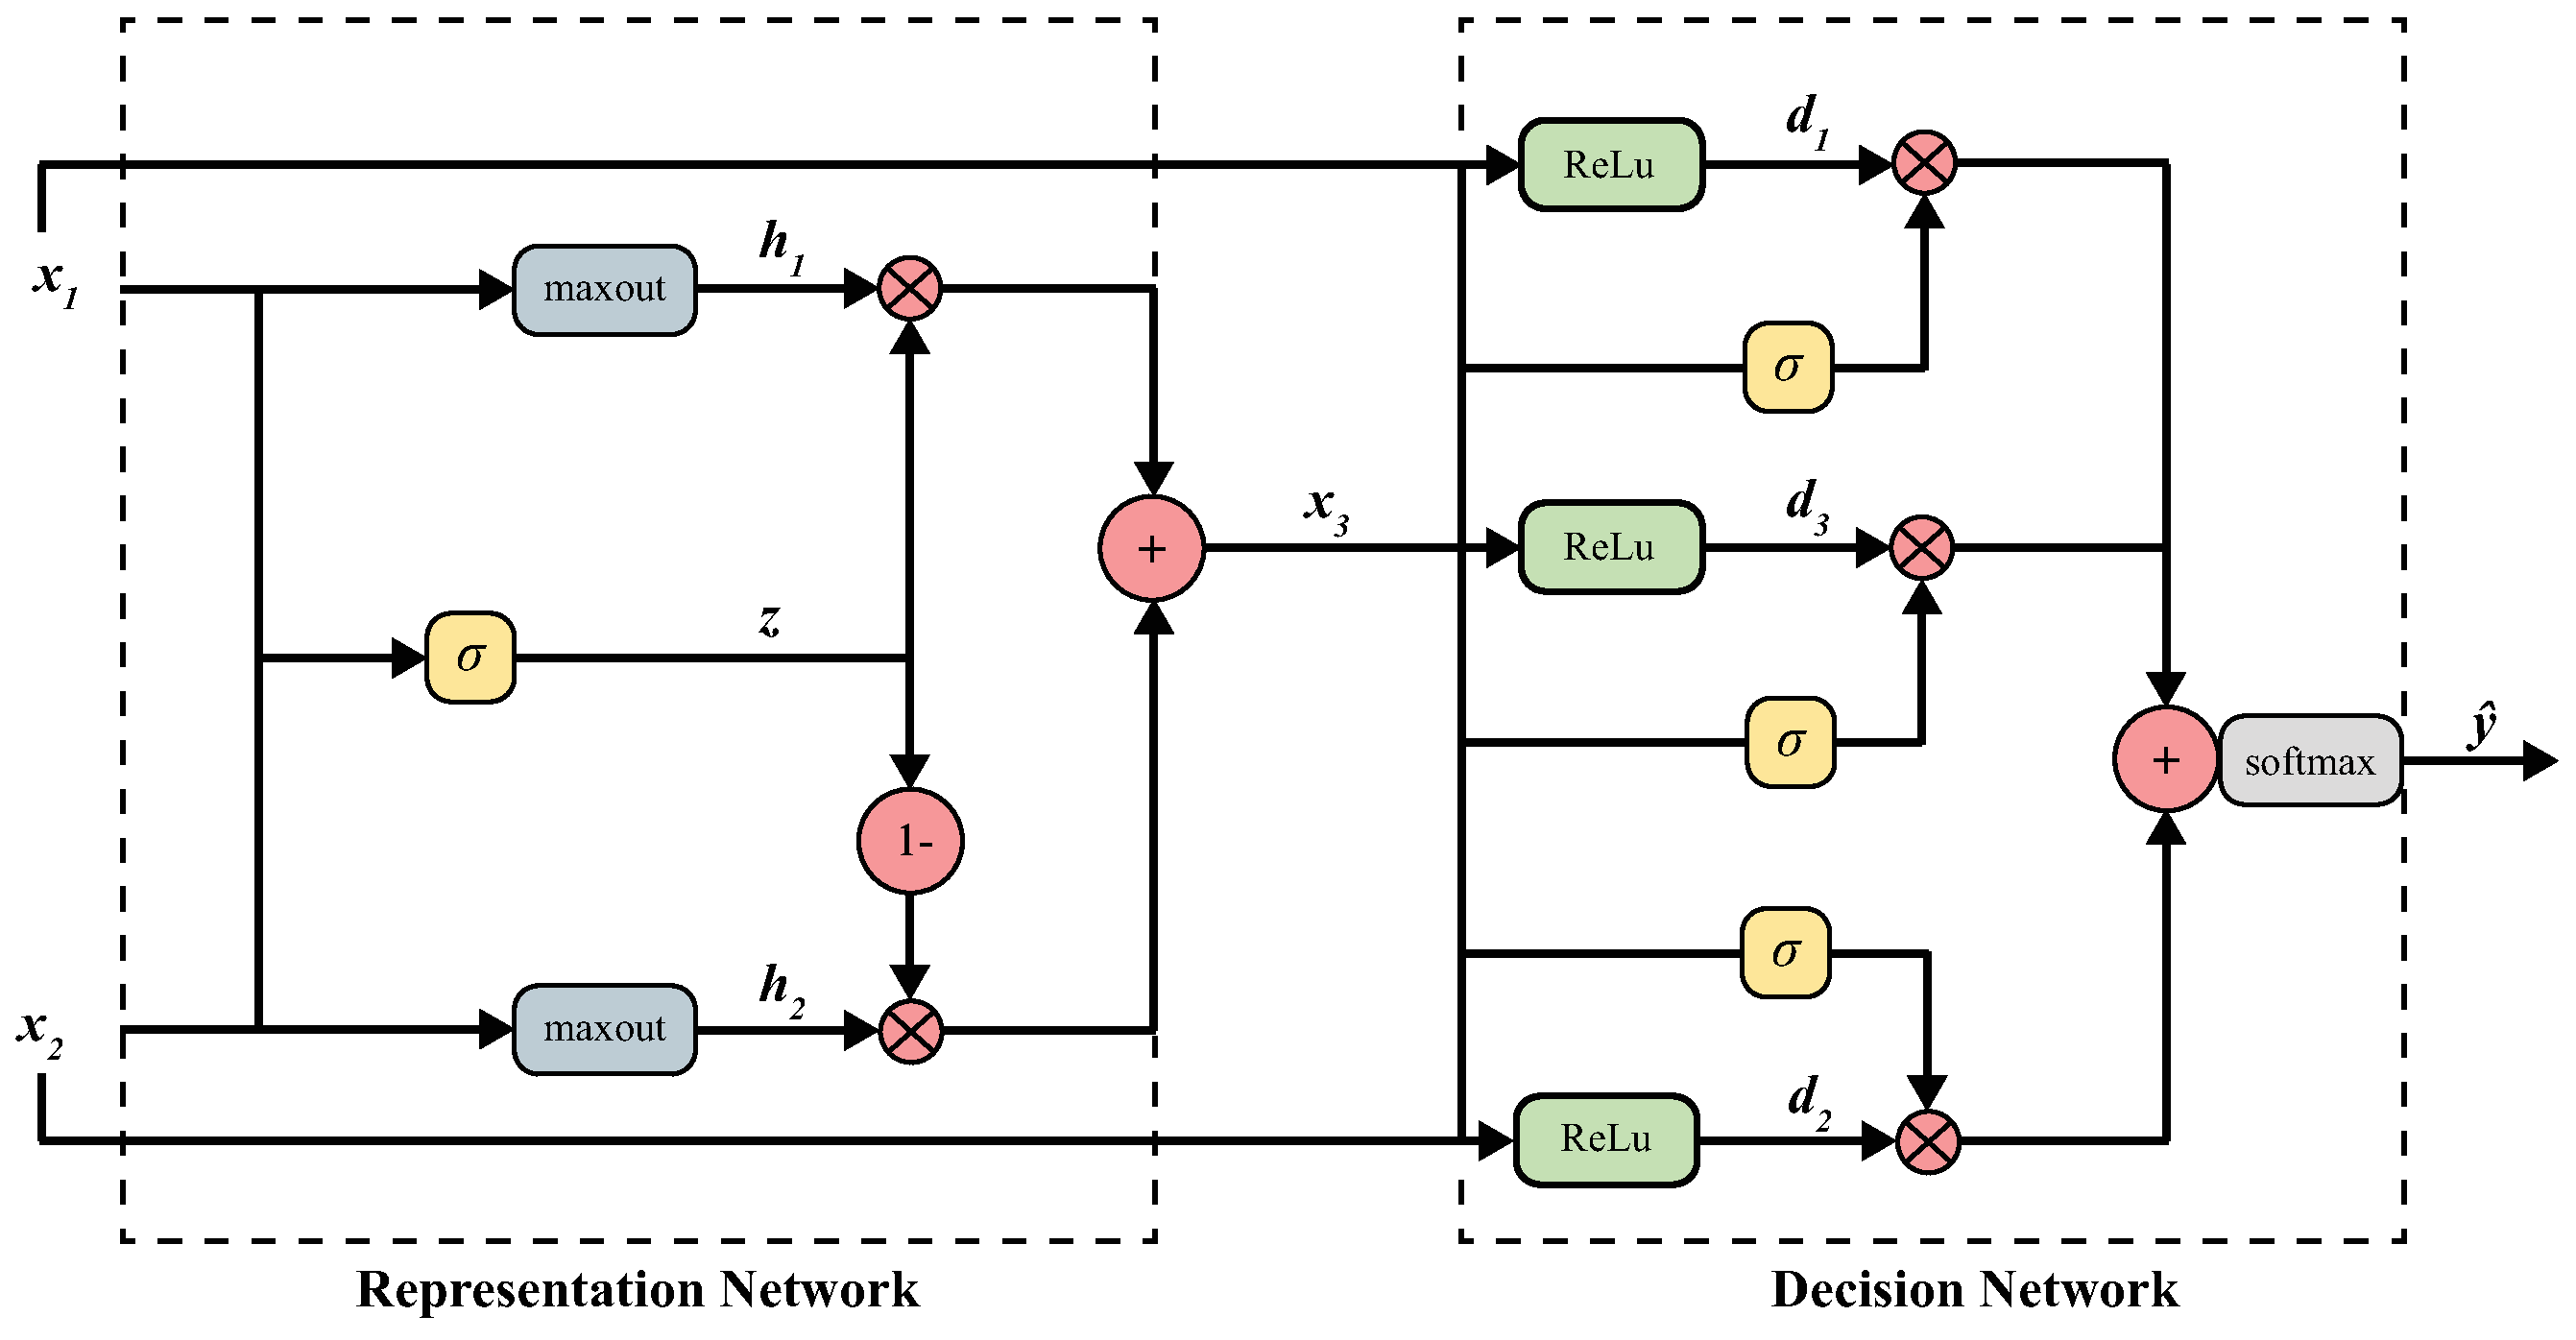
\includegraphics[width=\textwidth]{img/dGMU.eps}
    \caption{Deep Gated Multimodal Unit.}
    \label{fig:dgmu}
\end{figure}

\noindent
\textbf{Representation Network}

In this network, the input modalities learn a latent representation of the combined input data. Each modality becomes the input for a multilayer perceptron (MLP) with a maxout activation function, maxout$(\cdot)$ \cite{goodfellow2013maxout}. In Fig. \ref{fig:dgmu}, this produces $h_1 = \mathrm{maxout}(\theta_{h1} \cdot x_1)$ and $h_2 = \mathrm{maxout}(\theta_{h2} \cdot x_2)$, for modalities $x_1$ and $x_2$, respectively. Activated by the sigmoid activation function, $\sigma(\cdot)$, the gating neuron, $z = \sigma(\theta_z \cdot [x_1,x_2])$, ties both modalities and controls their contribution to the output of the unit. The output of the representation network is governed by the following equations:


\begin{align}
    h_1 &= \mathrm{maxout}(\theta_{h1} \cdot x_1)\notag\\
    h_2 &= \mathrm{maxout}(\theta_{h2} \cdot x_2)\notag\\
    z &= \sigma(\theta_z \cdot [x_1,x_2])\notag\\
    x_3(x_1,x_2;\Theta_R) &= z * h_1 + (1-z)*h_2,
\end{align}

\noindent
where latent space, $x_3(x_1,x_2;\Theta_R)$, depends on inputs $x_1$ and $x_2$, and $\Theta_R = \left\{\theta_{h1},\theta_{h2},\theta_{x3}\right\}$ is the set of parameters used for encoding the latent space.

\noindent
\textbf{Decision Network}

This network makes predictions based on all representations and learns to decide how decisions influence the activation of the output unit. Each representation from the representation network becomes the input to an MLP with a rectified linear unit (ReLU) activation function. Here, gating neuron $\sigma(\cdot)$ controls the untied contributions of decision gates $d_1$, $d_2$, and $d_3$. The decision network is governed by the following equation:

\begin{equation}
        \hat{y}(x_1,x_2,x_3;\Theta_D) = {\sum^{3}_{i=1}} \mathrm{ReLu}(\theta_{di} \cdot x_i)\sigma(\theta_{di} \cdot [x_1,x_2,x_3]),
    %$\Theta_D = \left\{W_{d1},W_{d2},W_{d3},W_{g1},W_{g2},W_{g3}\right\}$\\
\end{equation}

\noindent
where the network output, $\hat{y}(x_1,x_2,x_3;\Theta_D)$, depends on inputs $x_1$, $x_2$, and $x_3$, and $\Theta_D = \left\{\theta_{d1},\theta_{d2},\theta_{d3},\theta_{g1},\theta_{g2},\theta_{g3}\right\}$ is the set of network parameters used across the untied gates in the decision network.

%Internal gating neuron
%representation network
%decision network

\section{Training}

%majahan

The dGMU model parameters were learned with batch stochastic gradient descent with ADAM optimization \cite{kingma2014adam}. The training complexity was reduced by using a supervised pre-training scheme on the decision network \cite{mahajan2018exploring}. This method is used to initialize the parameters of the decision network to ease the training of the larger model, reducing computation time and increasing model robustness \cite{clune2013evolutionary}. The complete network was optimized using supervised fine-tuning with the connected sub-networks. During the training process, overfitting was controlled using dropout and $L_2$ regularization. For classification problems the global loss is computed using the softmax cross entropy loss as in Equation (\ref{eq:softmax}). With regularization, this results in the following global loss:

\begin{equation}
    \mathrm{Loss} = - \frac{1}{m}\sum_{i = 1}^{m}\sum_{j = 1}^{k} \lbrack y_{i,j} \log(\hat{y_{i,j}}) + (1 - y_{i,j})\log(1 - \hat{y_{i,j}}) \rbrack + \frac{\lambda}{2m} \sum_{j = 1}^{p}\sum_{k = 1}^{q}\Theta^{2}_{j,k}
\end{equation}

\section{Implementation}

The dGMU model was implemented with original code in Tensorflow version 1.11.0 on an Nvidia Tesla K80 GPU. With a high level of parallelization and batch training used during pretraining and finetuning, the model training takes a few minutes, and validation and testing is conducted in a matter of seconds.

The dGMU model benefits from the modularity of gated multimodal units. Accordingly, this architecture can be adapted using varying models for each modality depending on the application. As well, the decision network can be modified to accept inputs from more than two modalities while only resulting in a linear increase in the number of training weights. Furthermore, this model generates a latent space in between the representation network and the decision network. This offers an interesting avenue into investigating the biological significance of the fused latent representation. 